% Options for packages loaded elsewhere
\PassOptionsToPackage{unicode}{hyperref}
\PassOptionsToPackage{hyphens}{url}
%
\documentclass[
]{article}
\usepackage{lmodern}
\usepackage{amssymb,amsmath}
\usepackage{ifxetex,ifluatex}
\ifnum 0\ifxetex 1\fi\ifluatex 1\fi=0 % if pdftex
  \usepackage[T1]{fontenc}
  \usepackage[utf8]{inputenc}
  \usepackage{textcomp} % provide euro and other symbols
\else % if luatex or xetex
  \usepackage{unicode-math}
  \defaultfontfeatures{Scale=MatchLowercase}
  \defaultfontfeatures[\rmfamily]{Ligatures=TeX,Scale=1}
\fi
% Use upquote if available, for straight quotes in verbatim environments
\IfFileExists{upquote.sty}{\usepackage{upquote}}{}
\IfFileExists{microtype.sty}{% use microtype if available
  \usepackage[]{microtype}
  \UseMicrotypeSet[protrusion]{basicmath} % disable protrusion for tt fonts
}{}
\makeatletter
\@ifundefined{KOMAClassName}{% if non-KOMA class
  \IfFileExists{parskip.sty}{%
    \usepackage{parskip}
  }{% else
    \setlength{\parindent}{0pt}
    \setlength{\parskip}{6pt plus 2pt minus 1pt}}
}{% if KOMA class
  \KOMAoptions{parskip=half}}
\makeatother
\usepackage{xcolor}
\IfFileExists{xurl.sty}{\usepackage{xurl}}{} % add URL line breaks if available
\IfFileExists{bookmark.sty}{\usepackage{bookmark}}{\usepackage{hyperref}}
\hypersetup{
  pdftitle={Bike Challenge},
  pdfauthor={Sophie Manuel},
  hidelinks,
  pdfcreator={LaTeX via pandoc}}
\urlstyle{same} % disable monospaced font for URLs
\usepackage[margin=1in]{geometry}
\usepackage{graphicx}
\makeatletter
\def\maxwidth{\ifdim\Gin@nat@width>\linewidth\linewidth\else\Gin@nat@width\fi}
\def\maxheight{\ifdim\Gin@nat@height>\textheight\textheight\else\Gin@nat@height\fi}
\makeatother
% Scale images if necessary, so that they will not overflow the page
% margins by default, and it is still possible to overwrite the defaults
% using explicit options in \includegraphics[width, height, ...]{}
\setkeys{Gin}{width=\maxwidth,height=\maxheight,keepaspectratio}
% Set default figure placement to htbp
\makeatletter
\def\fps@figure{htbp}
\makeatother
\setlength{\emergencystretch}{3em} % prevent overfull lines
\providecommand{\tightlist}{%
  \setlength{\itemsep}{0pt}\setlength{\parskip}{0pt}}
\setcounter{secnumdepth}{5}
\usepackage{fancyhdr}
\pagestyle{fancy}
\usepackage{dsfont}
\usepackage{subfig}
\usepackage{amsmath}
\usepackage{amssymb}
\usepackage{amsthm}
\usepackage{amsmath}
\usepackage{dsfont}
\ifluatex
  \usepackage{selnolig}  % disable illegal ligatures
\fi

\title{Bike Challenge}
\author{Sophie Manuel}
\date{}

\begin{document}
\maketitle

Nous cherchons dans ce challenge à prédire le nombre de vélos qui
passeront à Albert 1er à Montpellier, le 2 Avril entre minuit et 9h.
Pour cela on utilisera les données collectée depuis 1 an sur lesquelles
nous ferons une régression linéaire.

\hypertarget{le-jeu-de-donuxe9es}{%
\section{Le jeu de donées}\label{le-jeu-de-donuxe9es}}

Pour exploiter le jeu de données il fallait le modifier. Nous devons
débuter avec le téléchargement des données avec le package
\texttt{download}, grâce auquel nous pouvons avoir une mise à jour des
données immédiatement.

Puis, nous avons pu retirer les lignes et les colonnes vides ou
inintéressantes pour ce challenge. Nous avions donc 3 colonnes :
``Date'', ``Heure'', ``Total de la journée''.

Une fois que tout cela est fait, nous pouvons procéder à la sélection
des données en prenant que celles étant entre minuit et 9h comme
demandé.

Ensuite, grâce au package \texttt{pandas} nous avons changer le format
des dates pour les mettre au format international afin de pouvoir les
traiter plus facilement. De plus, il a permit de grouper les données par
jour avec la fonction \texttt{groupby}du package. Pour grouper ces
variables, nous avons choisi de ne prendre que la dernière données du
jour dans la colonne ``Total de la journée'', car elle représente le
nombre de vélos passés entre minuit et l'heure en question. Nous avons
pu utiliser \texttt{.last()} pour grouper les données car elles étaient
rentrées dans l'ordre chronologique, si ce n'était pas le cas nous
aurions dû utiliser le maximum.

\hypertarget{ruxe9gression-et-pruxe9diction}{%
\section{Régression et
prédiction}\label{ruxe9gression-et-pruxe9diction}}

Enfin, nous avons pu faire une régression linéaire avec la fonction
\texttt{lingress} du module \texttt{scipy.stats}. Nous avons trouvé
\(\hat\beta_0=67.12\) pour l'ordonnée à l'origine et
\(\hat\beta_1=0.49\) pour la pente à \(10^{-2}\) près. Donc : \[
 \hat y = \hat\beta_0 + \hat\beta_1 \times x = 67.12 + 0.49 \times x
 \] Il permet de prévoir qu'il y aurait 157 vélos qui passeraient le 2
avril entre minuit et 9h, arrondi au vélo près. Cependant, lorsque nous
regardons le \(R^2\) on prévoit que ce modèle n'est pas très bon pour de
la prédictions sur nos données. Il est de \(6\%\).

\newpage

Voici le graphique que nous avons obtenu:

\begin{figure}
\centering
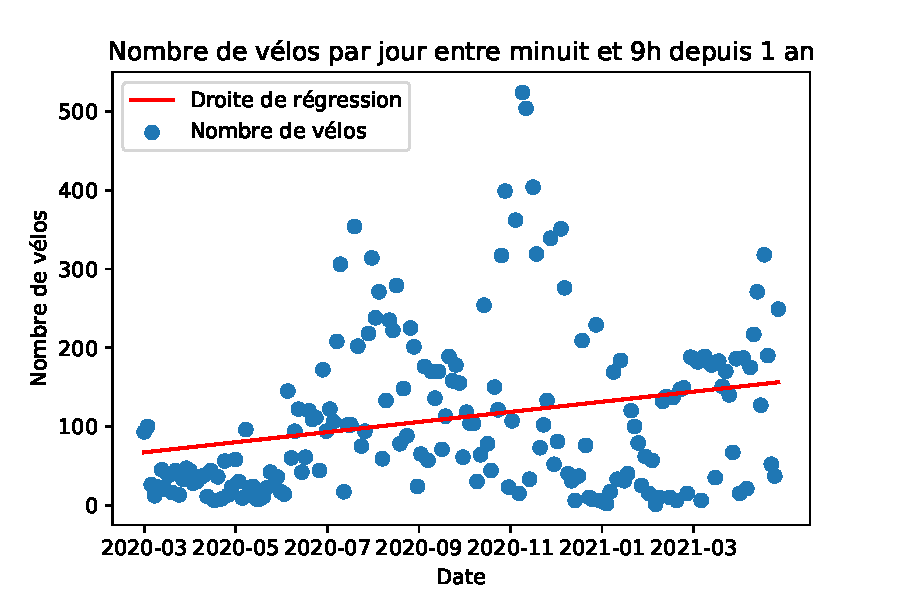
\includegraphics{Graph regression lineaire.pdf}
\caption{Graphique regression lineaire}
\end{figure}

\hypertarget{critiques-du-moduxe8le}{%
\subsection{Critiques du modèle}\label{critiques-du-moduxe8le}}

\begin{verbatim}
On constate que la variance des données est très grande au cours du temps. Effectivement entre juillet et décembre 2020 on remarque 2 pics, mais les données sont trop nombreuses pour être de simples points abérants. Il y a sans doute un effet de saisonnalité que nous n'avons pas analysé.
\end{verbatim}

De plus, la courbe est clairement faussée par les données avant le mois
de juin 2020 car c'était durant le premier confinement qui était assez
strict. Celles-ci on un effet de levier sur la droite.

Pour conclure, ce modèle (bien qu'imparfait) prédit qu' il y aura 157
vélos qui passeront à Albert 1er à Montpellier, le 2 Avril entre minuit
et 9h.

Lien du dépot Github :
\url{https://github.com/SophieManuel/Bike_Challenge}

\end{document}
